\documentclass[10pt,twocolumn]{article}

% use the oxycomps style file
\usepackage{oxycomps}
\usepackage{csquotes}

% usage: \fixme[comments describing issue]{text to be fixed}
% define \fixme as not doing anything special
\newcommand{\fixme}[2][]{#2}
% overwrite it so it shows up as red
\renewcommand{\fixme}[2][]{\textcolor{red}{#2}}
% overwrite it again so related text shows as footnotes
%\renewcommand{\fixme}[2][]{\textcolor{red}{#2\footnote{#1}}}

% read references.bib for the bibtex data
\bibliography{references}

% include metadata in the generated pdf file
\pdfinfo{
    /Title (Junior Comprehensive Proposal)
    /Author (Julianne Yotov)
}

% set the title and author information
\title{Final Senior Comprehensive Paper}
\author{Julianne Yotov}
\affiliation{Occidental College}
\email{jyotov@oxy.edu}

\begin{document}

\maketitle

\section{Problem Statement}

My senior comprehensive project was to create a website for high school and college students taking introductory level courses in computer programming that offers a variety of coding exercises through which users learn how to effectively test code. My inspiration for this project primarily comes from CodingBat \cite{CodingBat}, a website with coding exercises for both Python and Java. My initial motivation behind this project was largely due to my own experience with taking AP Computer Science in high school. I struggled with many of the coding projects that we were assigned and found that this was largely due to my lack of understanding of basic foundational concepts, such as how to write a proper for loop. When I started doing CodingBat exercises, I found that I enjoyed working through the exercises and gained a lot of confidence in the process. I particularly liked that CodingBat’s pre-written test cases allowed me to easily spot patterns in the cases that were failing, which allowed me to find errors in my code independently. By working on these problems, I was able to put certain skills, such as creating arrays and writing nested loops, into use when working on larger coding projects that involved writing classes with multiple methods.

I was also inspired to pursue a project related to computer science education from my experience remotely tutoring two students in Python, a sixth grade student with some previous experience learning Python, and a high school student with no previous coding experience. From their feedback throughout our sessions, I started to gain a sense of which educational resources were effective. I sometimes started sessions by presenting a new concept, but ensured that they had the opportunity to do a lot of coding practice. Both of them expressed that they enjoyed working through exercises in CodingBat and felt a sense of accomplishment when all of the test cases would pass. However, I found that I struggled to teach them about the importance of testing code outside of CodingBat and did not know how to best present examples. When we worked on writing test cases, whether for a short method or for an entire game we made, I found that my students often didn’t quite know how to best structure their test cases to ensure that they were covering edge cases. 

I began to realize that I myself had never spent a lot of time learning how to properly test my code. It wasn’t until I came to Occidental and took COMP 181 (Advanced Programming) that I actually remember learning about testing, and we had one assignment specifically devoted to testing code, while the importance of it was emphasized throughout the course. I feel that I would have benefited from this level of instruction in high school given how I struggled with coding and understanding my code's errors. This is what ultimately led me to decide to emphasize testing for this project, as this allowed me to ensure that I had a specific focus and goal that I wanted to achieve. I aimed to design my website in such a way that users find the task enjoyable rather than extremely tedious, and that they come to see testing as something that is somewhat similar to editing an essay; it allows you to find issues in your code and fix them. I hope to emphasize the importance of proper testing in a way that ensures that users will be able to take the concepts that they have learned from using my website and apply them to future coding-related projects. I feel that creating this educational website that teaches users how to write test cases for their code can be particularly useful to high school students taking coding classes, undergraduate college students taking introductory computer programming courses, and students taking courses that require coding for a subject area other than computer science. Therefore, this will be the primary audience for my project, and I will be seeking feedback from these groups while creating my website.

Additionally, many students who may be interested in taking classes in computer programming may not have the opportunities to take any computer science courses in high school. If these students want to major in Computer Science or take some computer programming courses in college, then they may feel that they are at a disadvantage compared to their peers who had the opportunity to take computer science classes in high school. According to CalMatters, "Only 40\% of California high schools offer computer science classes" \cite{California}. This suggests that there are many students nation-wide who have very limited opportunities to learn computer programming in a classroom setting before college. This highlights the importance of free resources, as students interested in pursuing Computer Science may seek them out to prepare. While this website contains minimal instructional material and is mostly designed to be used by students taking a course that involves computer programming, I was also interested in creating a resource that could hypothetically be used by a larger group of people.

\section{Technical Background}

Due to the nature of my project, one of the most important aspects was deciding how to structure my website to emphasize testing. As previously stated, I structured my website based on CodingBat's design. However, CodingBat provides all of the test cases that are used to test a function. The goal of this resource is to allow the user to learn how to write their own unit tests. Many existing resources for computer science education teach introductory level concepts and have exercises for practice applying them, but there is often little information on how to test code. The exercises may simply be accompanied by solutions for users to check if they are struggling, but there is often no incentive for users to learn to come up with their own test cases. Unit testing refers to a testing technique in which \enquote{units}, which are small pieces of code, are tested to see if they are producing the intended outputs \cite{Unit}. In all of the exercises in this resource, all of the \enquote{units} to be tested are functions. There are other types of tests that focus on testing much larger chucks of code. For example, some tests are intended to test the functionality of entire applications. The goal of this resource is for users to get comfortable with effectively testing isolated functions.

This website was built with the Dash framework. Dash is built on top of the Plotly.js (for graphing) and React (for user interfaces) libraries. Dash allows you to easily implement UI elements like dropdowns, sliders and graphs directly using Python code. Dash apps consist of a Flask server that communicates with front-end React components using JSON packets over HTTP requests and are written in Python; no HTML or JavaScript is needed. This is beneficial because the users can then define all functions using Python, which is typically the language covered in introductory level computer science courses. Dash apps consist of two components: the layout, which defines what the app looks like, and callback functions, which are called when an input component’s property changes so that the output can be updated \cite{Dash}.

\section{Prior Work}

As discussed in the Problem Statement section, I hope to emulate some of CodingBat’s elements within my project \cite{CodingBat}. As shown in Figure 1, the coding exercises are sorted into groups based on the concepts that they cover, including String, Array (for Java) or List (for Python), Logic (which include logic puzzles). When clicking on an exercise, the instructions are given, below which are listed a few examples of the expected outputs for certain inputs, as shown in Figure 2. The user can then type their code directly into the box below the function or method heading and run their code. Then, a series of test cases will appear, and it is noted whether each output matches the expected output or not, as shown in Figure 3. Finally, once all test cases pass (as in Figure 4), that exercise is marked as completed. CodingBat specifies a certain number of test cases (seven in the coding exercise shown in Figures 2, 3, and 4). While additional test cases are utilized, as demonstrated by the “other tests” row in Figures 3 and 4, the seven tests cover a variety of different cases, such as an empty string and strings with numbers. There are certain incentives to keep users engaged. Completing any three exercises in a section earns the user a star, and earning one star in each section earns the user a 5-star badge, while earning two stars and five stars in each section earns the user a 10-star badge and 25-star badge, respectively.

\begin{figure}
    \centering
    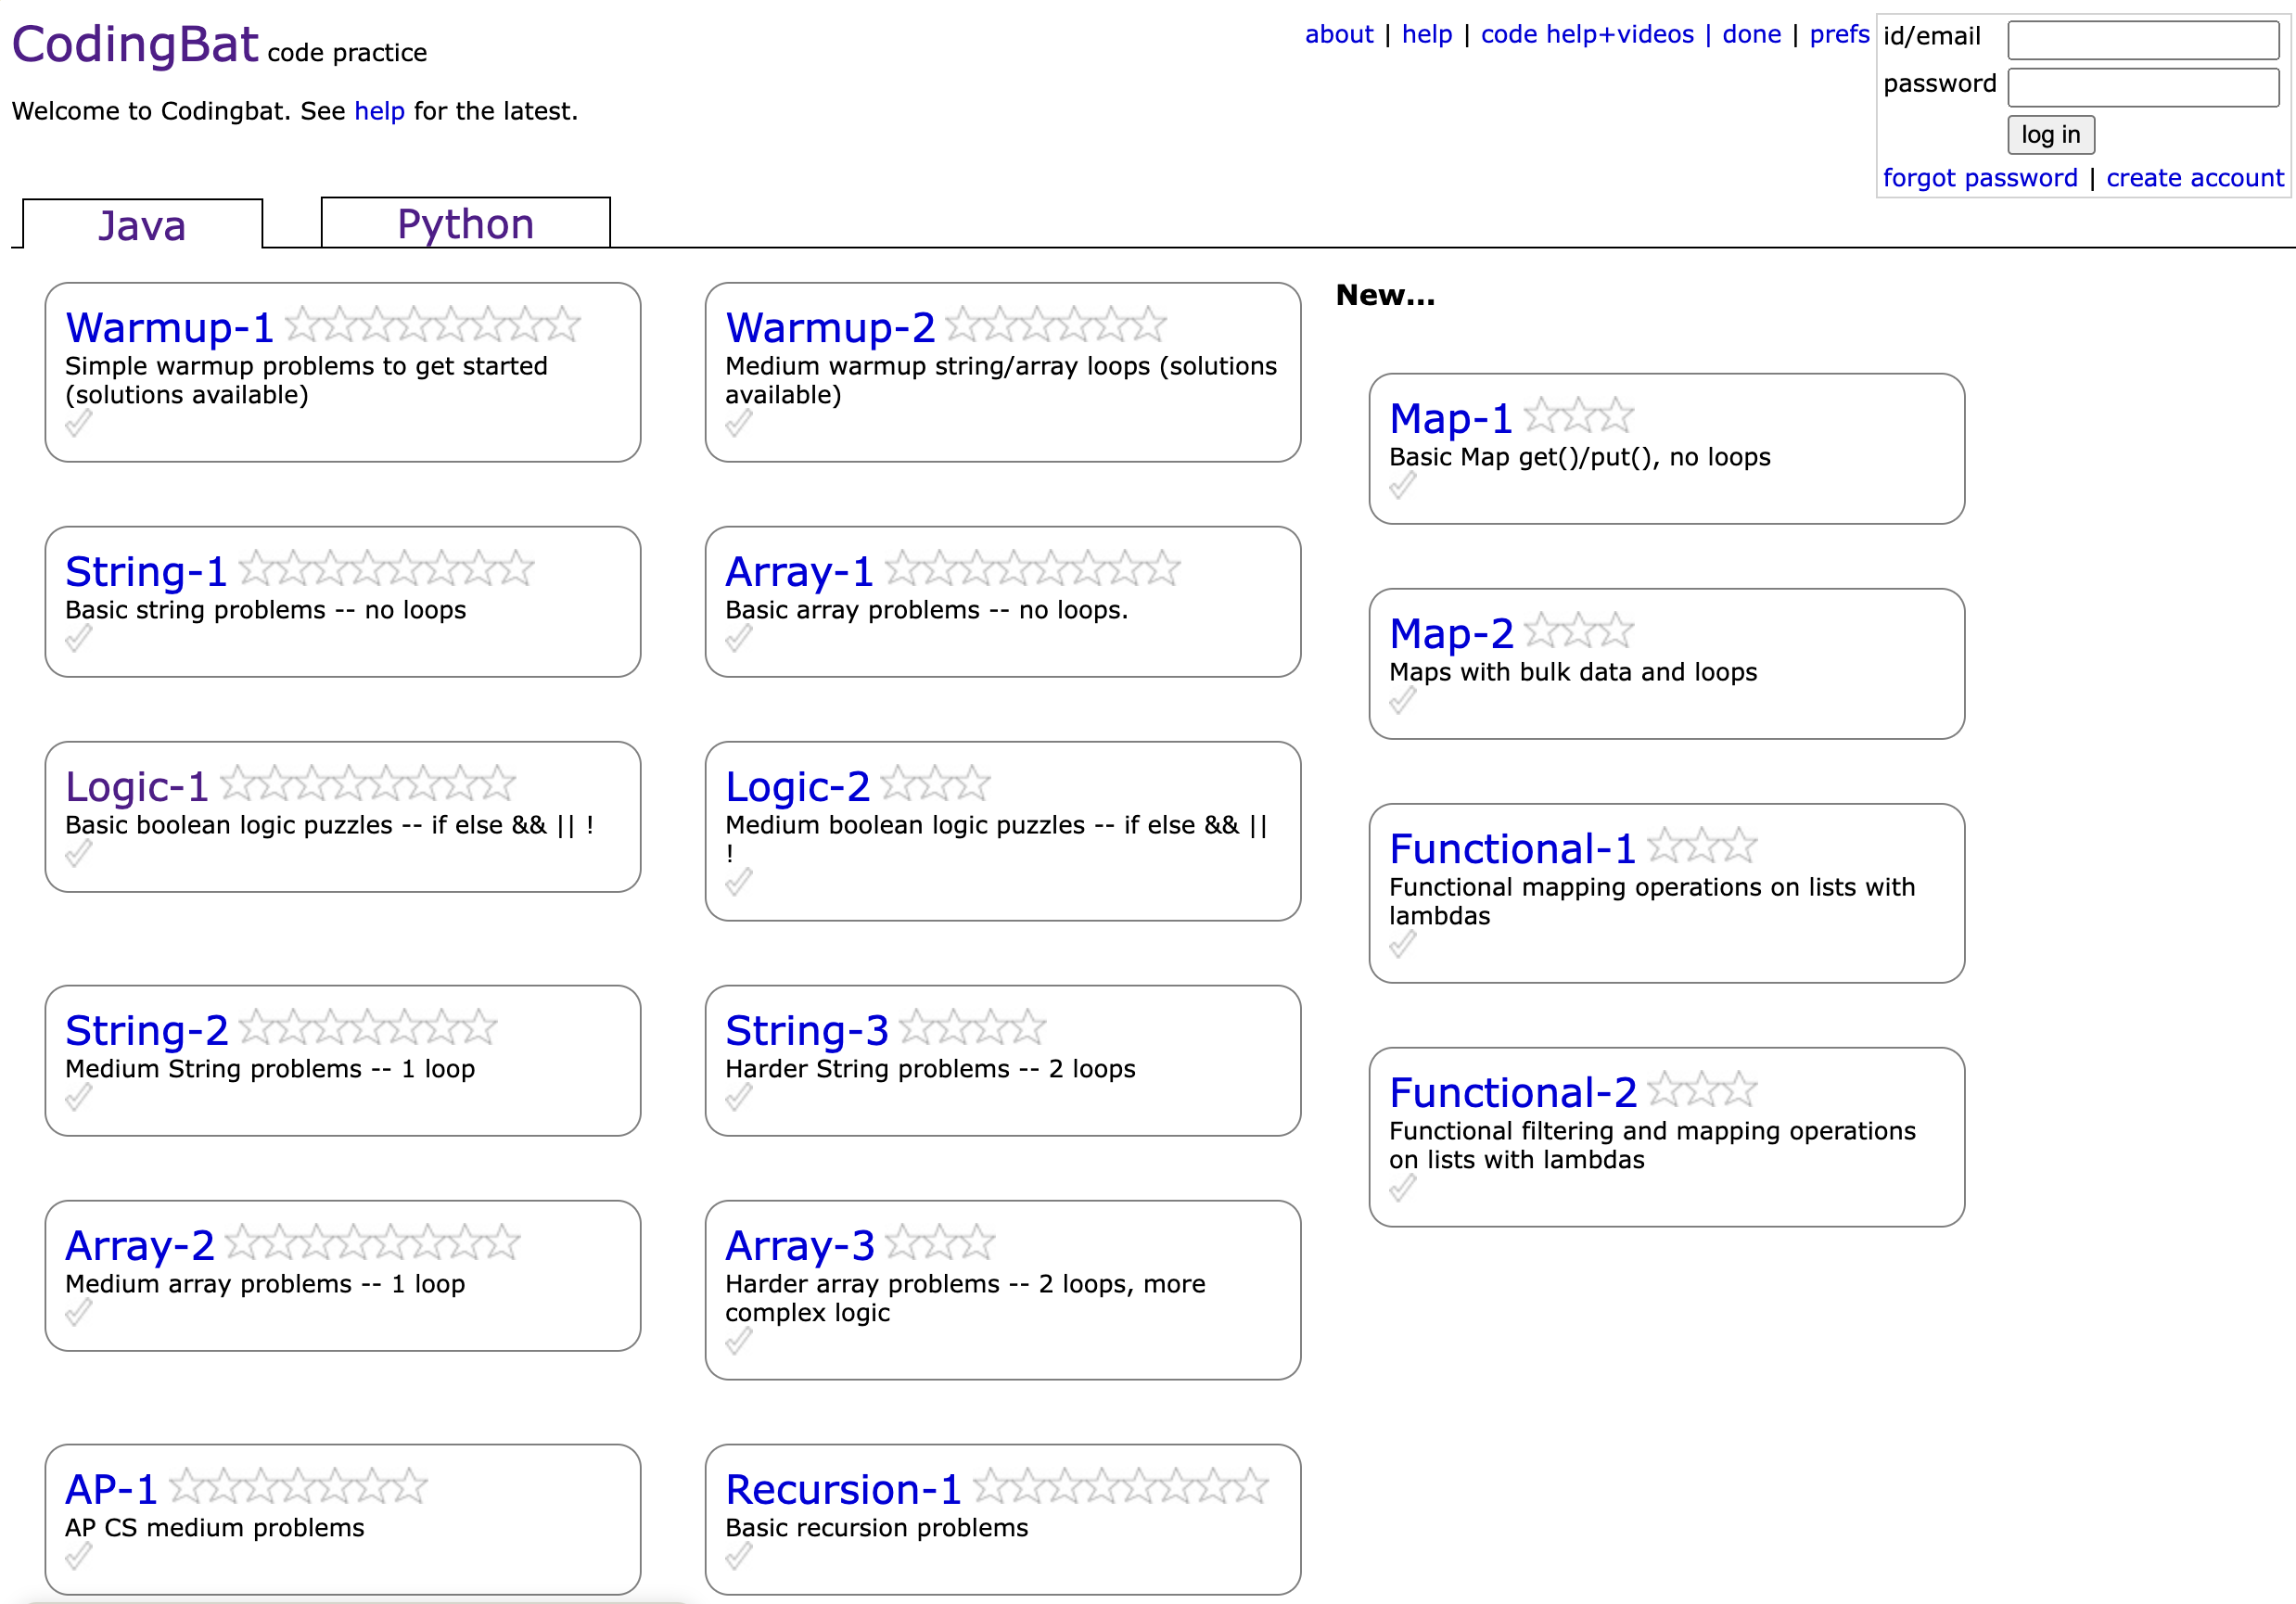
\includegraphics[width=.95\linewidth]{CodingBat0.png}
    \caption{
        Home page of CodingBat's coding exercises for Java.
    }
    \label{fig:first-page}
\end{figure}

\begin{figure}
    \centering
    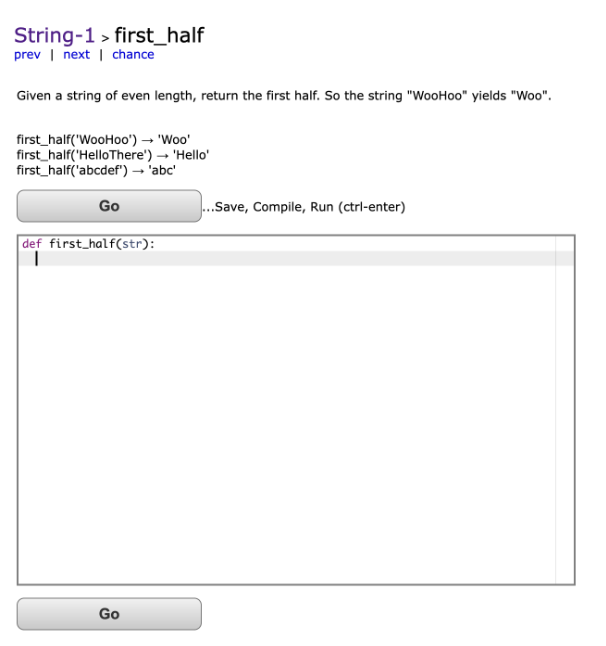
\includegraphics[width=.95\linewidth]{CodingBat1.png}
    \caption{
        One Python coding exercise in CodingBat.
    }
    \label{fig:first-page}
\end{figure}

\begin{figure}
    \centering
    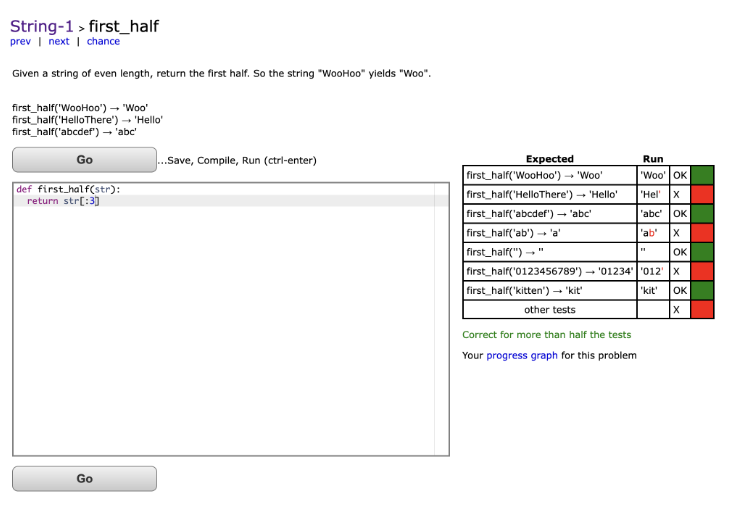
\includegraphics[width=.95\linewidth]{CodingBat2.png}
    \caption{
        Test cases for this function. Some test cases have failed, indicating an error in the code.
    }
    \label{fig:first-page}
\end{figure}

\begin{figure}
    \centering
    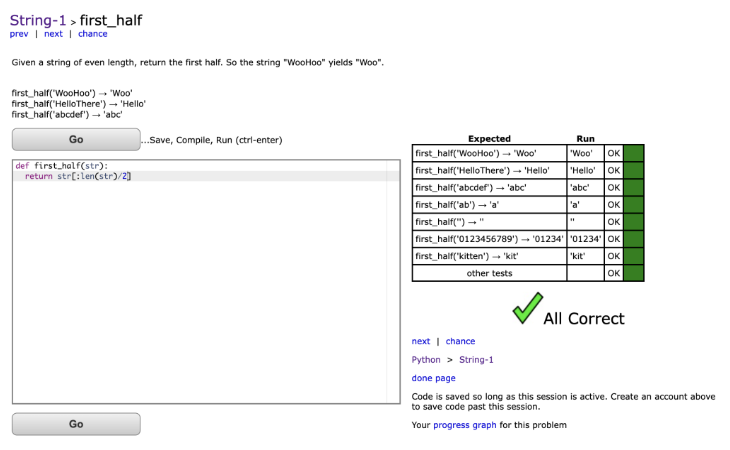
\includegraphics[width=.95\linewidth]{CodingBat3.png}
    \caption{
        All test cases have passed for this function.
    }
    \label{fig:first-page}
\end{figure}

Two primary conferences relating to computer science education are the Special Interest Group on Computer Science Education (SIGCE) and International Computing Education Research (ICER). One paper from ICER’s 2023 conference, titled “Evaluating Beacons, the Role of Variables, Tracing, and Abstract Tracing for Teaching Novices to Understand Program Intent” discusses the importance of “program comprehension,” stating that “Skill in program comprehension is undoubtedly necessary to be a strong programmer. “Explain in Plain English” (EiPE) questions capture an important aspect of students’ program comprehension ability: the capacity to identify the overall purpose or intent of a piece of code [18]. This competency to explain code is not only useful on its own—it [has] also been consistently found to correlate with other programming skills, like code tracing and writing [9, 23, 25], suggesting that similar knowledge underlies all of these abilities” \cite{Teaching}. While this paper is not related to teaching students how to test their code, its discussion on methods to determine students’ comprehension of code provides an important set of guidelines for my website. For instance, rather than asking students to immediately dive into writing code and test cases to test it, it is helpful to have them answer certain questions in written English as a method of brainstorming. This will not only allow users to take a moment to understand the exercise and what the expected output for a given input should be. They will be able to think through their code and what test cases will allow them to ensure that their code is functioning as intended.

Another paper relevant to this project, titled “Test-Driven Learning: Intrinsic Integration of Testing into the CS/SE Curriculum,” discusses the concept of “test-driven learning (TDL),” which they define as “...an approach to teaching computer programming that involves introducing and exploring new concepts through automated unit tests. TDL offers the potential of teaching testing for free, of improving programmer comprehension and ability, and of improving software quality both in terms of design quality and reduced defect density.” The authors define the basic principles of TDL as: (1) “teach[ing] by example,” (2) “present[ing] examples with automated tests,” and (3) “start[ing] with tests.” They expand on these concepts; the first two points are connected, as showing students examples with automated tests is an instance of teaching by example: “Teaching by example has a double meaning in TDL. First TDL encourages instructors to teach by presenting examples with automated tests. Second, by holding tests in high regard and by writing good tests, instructors model good practices that contribute to a number of positive results. Students tend to emulate what they see modeled. So as testing becomes a habit formed by example and repetition, students may begin to see the benefits of developing software with tests and be motivated to write tests voluntarily.” The authors go on to expand on what it means to “start with tests,” as TDL can utilize a test-first or test-last approach: “The third aspect of TDL suggests a test-first approach. TDL could be applied in either a test-first or a test-last manner. With a test-last approach, a concept would be implemented, then a test would be written to demonstrate the concept’s use and behavior. With a test-first approach, the test would be written prior to implementing a concept. By writing a test before implementing the item under test, attention is focused on the item’s interface and observable behavior” \cite{Test-driven}. This paper provides useful guidelines for how to implement test-driven learning, which is certainly something that my project will utilize. Additionally, the test-first approach suggests that it may be helpful for my website to have users write some test cases before writing their code, while also letting them write additional ones later if needed. Doing so can allow users to take time to fully consider the instructions and expected behavior of the function or method before actually writing it.

Another paper discussing the test-first approach, titled “Rethinking Computer Science Education from a Test-first Perspective,” describes the importance of having students submit test cases along with their code for assignments. The author states that “...most undergraduate curricula focus on developing program application and synthesis skills (i.e., writing code), primarily acquired through hands-on activities.” However, many students don’t necessarily appreciate the complexity of an assignment from testing with no genuine strategy; according to the author, “Particularly during freshman and sophomore courses [for undergraduates], and occasionally much later, a student may believe that once the code she has written compiles successfully, the errors are gone. If the program runs correctly on the first few runs she tries, it must be correct. If there is a problem, maybe by switching a few lines around or tweaking the code by trial and error, it can be fixed.” This means that students often complete their coding assignments “without developing a broader view, which only reinforces approaches that will handicap their performance in more advanced courses.” Therefore, it is essential that students understand the importance of testing early on and work to develop those skills as they progress through computer programming courses. This paper focuses on developing “... a vision of a test-first-inspired educational strategy: systematically supporting test-first programming from the beginning to ensure students acquire the necessary comprehension and analysis skills needed to support effective programming” \cite{Test-first}. Just like the previous paper, this paper also demonstrates the effectiveness of having students write tests before writing code for the actual assignment, as it ensures that they take the time to understand the instructions.

\section{Methods}

The first step when starting to create this resource was to familiarize myself with the Dash framework. Creating a text box in which the user can write their code was quite simple. The more challenging aspect was figuring out how to handle the test cases that the user would also write. Initially, I experimented with Dash's AG Grid. An AG Grid is a data grid with many features that allow for grouping and and filtering. Ultimately, this became too challenging to implement, and Dash's DataTable became a much simpler alternative. The DataTable is interactive and allows for the user to type inputs directly into it \cite{Dash}. Thus, the user can type in their unit tests, one per row, into the DataTable. Then, the output is displayed in the column directly to the right based on the function defined by the user.

I split up the functions into five categories: Warmup Exercises, String Exercises, List Exercises, For Loop Exercises, and While Loop Exercises. Each category has three functions total. None of the functions are meant to be incredibly challenging or require many lines of code. For many of them, there are many different ways to define the function, some of which may require a lot less code than others. Below is a detailed explanation of each function and a justification for what the user is learning:

\begin{itemize}
    \item{Warmup Exercises}
    \begin{itemize}
        \item{add: This exercise asks the user to define a function that adds two integers and returns their sum. This is the simplest function, and the main goal is to help the user familiarize themselves with the layout and how to input their unit tests.}
        \item{even\_odd: This exercise asks the user to define a function that returns 'Even' if the integer argument is even and 'Odd' if it is odd. The goal of this exercise is to teach or remind the user how to check if an integer is even or odd using the modulo operator.}
        \item{days\_in\_month: This exercise asks the user to define a function that returns the number of days in a given month. There are two arguments, one which is a string representing the month \enquote{January}, \enquote{February}, etc.). The second is a boolean argument that is True if it is a leap year and false otherwise. The goal of this exercise is to teach or remind the user how to write a chunk of code consisting of and if statement, multiple elif statements, and and else statement. Also, the user should return \enquote{Invalid month} if the month argument isn't formatted correctly (for example, if it's another word or if the month is written with a lowercase letter). This will hopefully serve as a reminder to handle unexpected inputs.}
    \end{itemize}
    \item{String Exercises}
    \begin{itemize}
        \item{first\_last: This exercise asks the user to define a function that takes a String argument and returns the first and last character. Additionally, if the string is empty, it should return an empty string, and if the string has one character, then it should return that character twice. The goal of this exercise is to teach or remind the user how to check the length of a String, access the first and last characters of a string, and concatenate strings or characters together.}
        \item{reverse: This exercise asks the user to define a function that takes a String argument and returns the reverse of it. For example, reverse(\enquote{Hello}) should return \enquote{olleH}. If the argument is an empty string, then the function should return an empty string. The goal of this exercise is to challenge the user to experiment with different ways to define the function. Ideally, the user is able to eventually write a one-line return statement for strings that are not empty: return word[::-1].}
        \item{repeat\_first: This exercise asks the user to define a function that takes a String argument and returns a new string made of 3 copies of the first 2 characters of the original string. 
        For this function, the String length should be at least two, so there is no need to test words that are shorter than two letters. The goal of this exercise is to tech or remind the user how to slice Strings in Python and concatenate Strings (either by adding multiple Strings together or multiplying a given String by an integer).}
    \end{itemize}
    \item{List Exercises}
    \begin{itemize}
        \item{equal\_first\_last: This exercise asks the user to define a function with two arguments, a list of integers and an integer and to return True if the first element and the last element of the list are both equal to the integer and False otherwise. Additionally, the function should return False if the list is empty. The goal of this exercise is to teach or remind the user how to check the length of a list and access the first and last elements of a list.}
        \item{middle\_values: This exercise asks the user to define a function with two arguments, both lists of integers, each of odd length, and return a new list of length two containing their middle elements. The goal of this exercise is to teach or remind the user how to access the middle element of a list with an odd number of elements and create a new list.}
        \item{rotate\_right: This exercise asks the user to define a function with a list argument of length 3 and to return an array with the elements \enquote{rotated right} so that ['a', 'b', 'c'] yields ['c', 'a', 'b']. Thus, all test cases should have list arguments that are exactly length 3. The goal of this exercise is to teach or remind the user how to create a new list and define initialize its elements.}
    \end{itemize}
    \item{For Loop Exercises}
    \begin{itemize}
        \item{count: This exercise asks the user to define a function that has two arguments: a list and item and return the number of times that the item occurs in the list. The list can have elements of different data types, including integers, Strings, and floating point numbers. The goal of this exercise is to teach or remind the user how to iterate through the elements of a list using a for loop.} 
        \item{triple\_chars: This exercise asks the user to define a function that takes a String argument  and returns a string where for every character in the original String is repeated three times. For example, if the argument is \enquote{Hello}, the output should be \enquote{HHHeeellllllooo}. The goal of this exercise is to teach or remind the user how to iterate through the characters of a String using a for loop.}
        \item{draw\_star\_triangle: This exercise asks the user to define a function that draws a isosceles triangle using the letter 'o' of height equal to the integer argument. For example, if this argument is 5, the function should output a triangle with one 'o' in the first row, two in the second row, five on the fifth row, four on the sixth row, and one on the ninth row. The goal of this exercise is to teach or remind the user when it's necessary to use more than one for loop and how to increment and decrement the values iterated through in the for loop.}
    \end{itemize}
    \item{While Loop Exercises}
    \begin{itemize}
        \item{five\_mults: This exercise asks the user to define a function that returns a list of the first five multiples of an integer using a while loop. The goal of this exercise is to allow the user to practice using a while loop, as this exercise may be more intuitive to solve using a for loop.}
        \item{in\_half: This exercise asks the user to return the number of times a given integer can be divided by 2 before it is less than or equal to 10. The goal of this exercise is to practice using a while loop where it is necessary to \enquote{update} the value of the argument so that the while loop eventually terminates.}
        \item{sum: This exercise asks the user to return the sum of numbers in a list using while loop. Once again, the goal of this exercise is to provide the user with practice using a while loop for an exercise that may be more intuitive to solve using a for loop.}
    \end{itemize}
\end{itemize}

Ultimately, the goal of all of these exercises is to encourage the user to go through multiple rounds of defining the function, writing the test cases, and modifying the function as needed until all test cases pass. As detailed in the Prior Work section, there are several benefits of emphasizing the importance of testing in introductory computer science education \cite{Test-first}\cite{Test-driven}\cite{Teaching}. While this resource does not in any way have users write their test cases before defining the function, it is designed so that users can edit their function after seeing which of their test cases pass and which don't (if any). Some functions also have examples of what a given test case should return, which will ideally encourage users to think of their own test cases while writing the function.

As detailed in the following section, input was gathered from both computer science professors and students who are Computer Science majors, have taken introductory level Computer Science courses, and/or have taken courses outside of the Computer Science department that require some level of programming.

\section{Evaluation Metrics}

My main goal with interviewing Computer Science professors who are teaching or have taught COMP 131 in the past was to hear a professor's perspective on how the course (and other introductory level Computer Science courses are taught) and hear their feedback on my project. I also asked them what they would consider to be a \enquote{comprehensive set of test cases} for a given function. Given my focus on emphasizing testing and research into current test-driven Computer Science education \cite{Test-driven}\cite{Test-first}\cite{Teaching}, I wanted to hear their thoughts on these educational models. One professor, who currently teaches COMP 131, emphasized that what is considered a \enquote{comprehensive set of test cases} is very dependent on the function itself. We discussed how some functions have only a finite number of possible test cases. For example, a function with two boolean arguments only has four possible test cases. However, many functions have an infinite number of test cases, and it is important to consider which test cases to write in order to comprehensively test the function. This professor suggested that for arguments that are numbers (integers or floating point numbers), that including zero is important. They also emphasized that it's difficult to catch all of the errors that people might make when defining functions and writing test cases, which is why its very difficult to write out all of the proper \enquote{error messages} that should be displayed to help the user understand their mistake. Currently, if a given row in the table where users can write test cases is empty (there is no test case written), there a generic error message displayed that tell the user that a String (the test case) was expected. This professor also suggested that I have the functions already written, but this is not ultimately something that I implemented. My goals was to allow users to find mistakes in their own code, rather than me having a incorrectly defined or correctly defined function so that they have to find certain \enquote{generic} errors that they might not make themselves.

Another professor that I spoke to has taught COMP 131 in the past. This professor agreed with most of what the previous professor said about what defines a \enquote{comprehensive set of test cases}. This professor asked me to consider encouraging users to structure their if/else statements such that the conditional that has the highest probability of being False is put first (in the if statement). I didn't ultimately end up including this in my project because I felt that I didn't have the time to adequately address all of the different \enquote{hints} that are useful for users to keep in mind. However, I feel that this would be a great addition to include when expanding my project in the future to better assist students.

I spoke to one more professor who has taught COMP 131 in the past. This professor mainly expressed how interesting they found the premise of my project and discussed their observations from teaching COMP 131. They mainly emphasized that they agreed that many students struggled with testing their code, since many assignments in COMP 131 (and other introductory level Computer Science class) have auto graders that automatically grade a student's work.

One student, who is a Computer Science major, shared that they do not recall learning how to write test cases in COMP 131 and ended up learning most of what they now know about testing from an internship. They felt that students could benefit from a resource that assists them with learning how to write test cases while also practicing some important concepts of coding. A student who is a Computer Science and Media Arts \& Culture major also shared similar sentiments. They also felt that they would have benefited from more practice writing test cases in their introductory Computer Science courses and felt that a resource like this would be helpful to students.

Another student, who is a Physics and Media Arts \& Culture major, shared that they have had to write code for classes in both of these majors. They have not taken a Computer Science Course at Occidental, and largely had to learn Python from their Physics research. They liked the overall layout of the the website but shared that they would find some additional feedback to be helpful for students on certain test cases that may be important to include but the user may have missed (particularly edge cases). They also shared that since some students who would benefit from this resource might not be taking any Computer Science courses, it would be helpful to write a little guide about what unit tests are. While I was not able to ultimately implement the \enquote{feedback} as I initially aimed to, I did include the guide on unit tests. In this guide, I also mentioned what edge cases to consider for different functions (such as an empty string for functions containing String arguments, an empty list for functions containing list arguments, and different combinations of negative numbers, zero, and positive numbers for functions with integer arguments). 

Finally, a few students who have taken introductory level Computer Science courses in college felt that the overall idea of the project was good and liked the setup. However, they expressed that the project would benefit from the additional feedback. According to all students, the current setup of the project is intuitive and generally achieves my project's aims. Every student I spoke to had many different ideas for ways to make this resource more useful for students. I ultimately was not able to properly implement any of the ideas that the students shared for ways to expand on the project, but I feel that I at least created something that could genuinely be used by students in introductory level Computer Science courses to supplement their learning. Students who would like more practice with computer programming who aren't in Computer Science courses may find that they need to also utilize additional outside resources to learn about some of the concepts that they may not have covered in their class.

\section{Results and Discussion}

Ultimately, I was able to create 15 exercises, sorted into five categories (Warmup Exercises, String Exercises, List Exercises, For Loop Exercises, and While Loop Exercises). None of these exercises are completely original, as these are relatively simple exercises. I drew inspiration from some of CodingBat's exercises \cite{CodingBat} and some exercises that I created during my past experience with tutoring. I did not copy any function directly, and made modifications to the exercise itself and the wording to ensure clarity. My aim was to make the functions manageable for students in introductory level Computer Science courses. However, most of the functions can be defined in ways that require a lot of code, as well as in a way that requires only a few lines. My goal is that the relative simplicity of the exercises encourages students to try defining the functions in multiple ways and to consider whether they can condense their code when they have correctly defined the function. However, I did not achieve my ultimate goal of developing a way to \enquote{guide} students with the test cases that they write by checking whether they've included a certain edge case and checking each function against certain pre-written test cases to make sure that the user didn't simply only choose test cases that happen to pass.

The home page of the website is shown in Figure 5 below. It includes five buttons that lead to the exercises related to those categories. There is also a short explanation of what unit tests are and what edge cases to possibly consider for different functions.
\begin{figure}
    \centering
    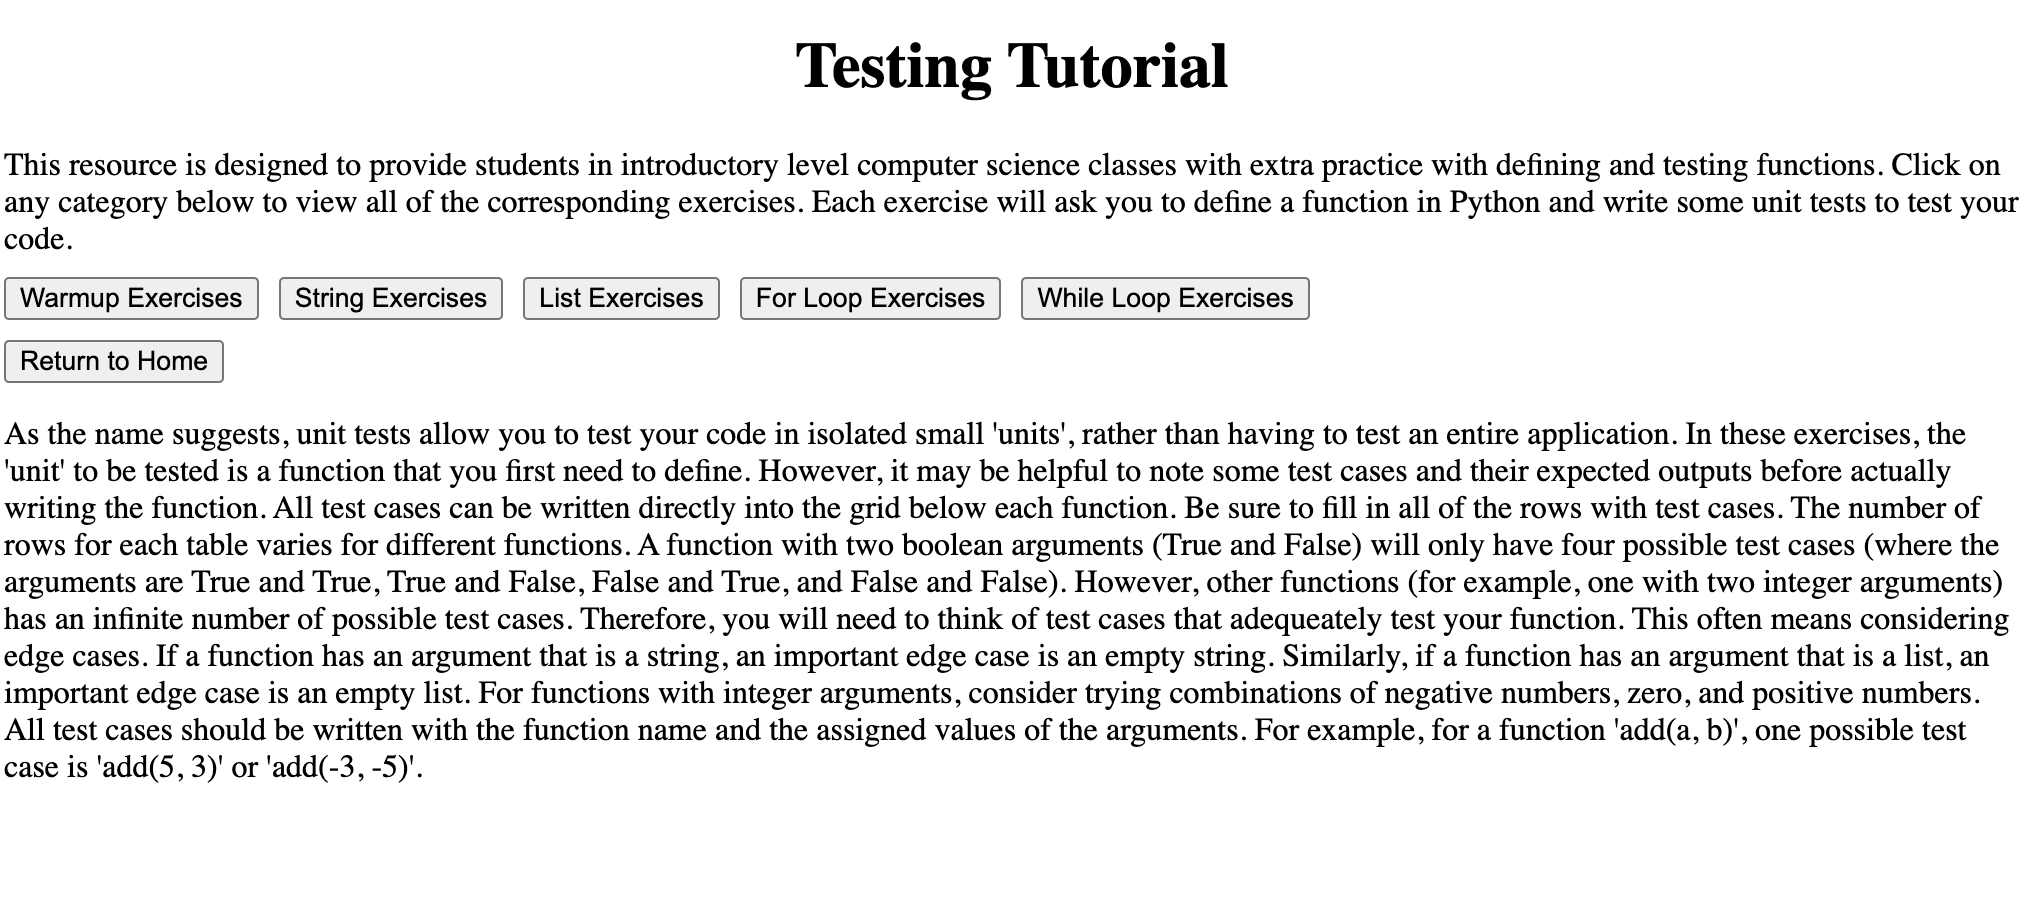
\includegraphics[width=.95\linewidth]{Home.png}
    \caption{
        Home page of my website.
    }
    \label{fig:first-page}
\end{figure}

Figure 6 shows the three exercises that are listed under \enquote{For Loop Exercises}.
\begin{figure}
    \centering
    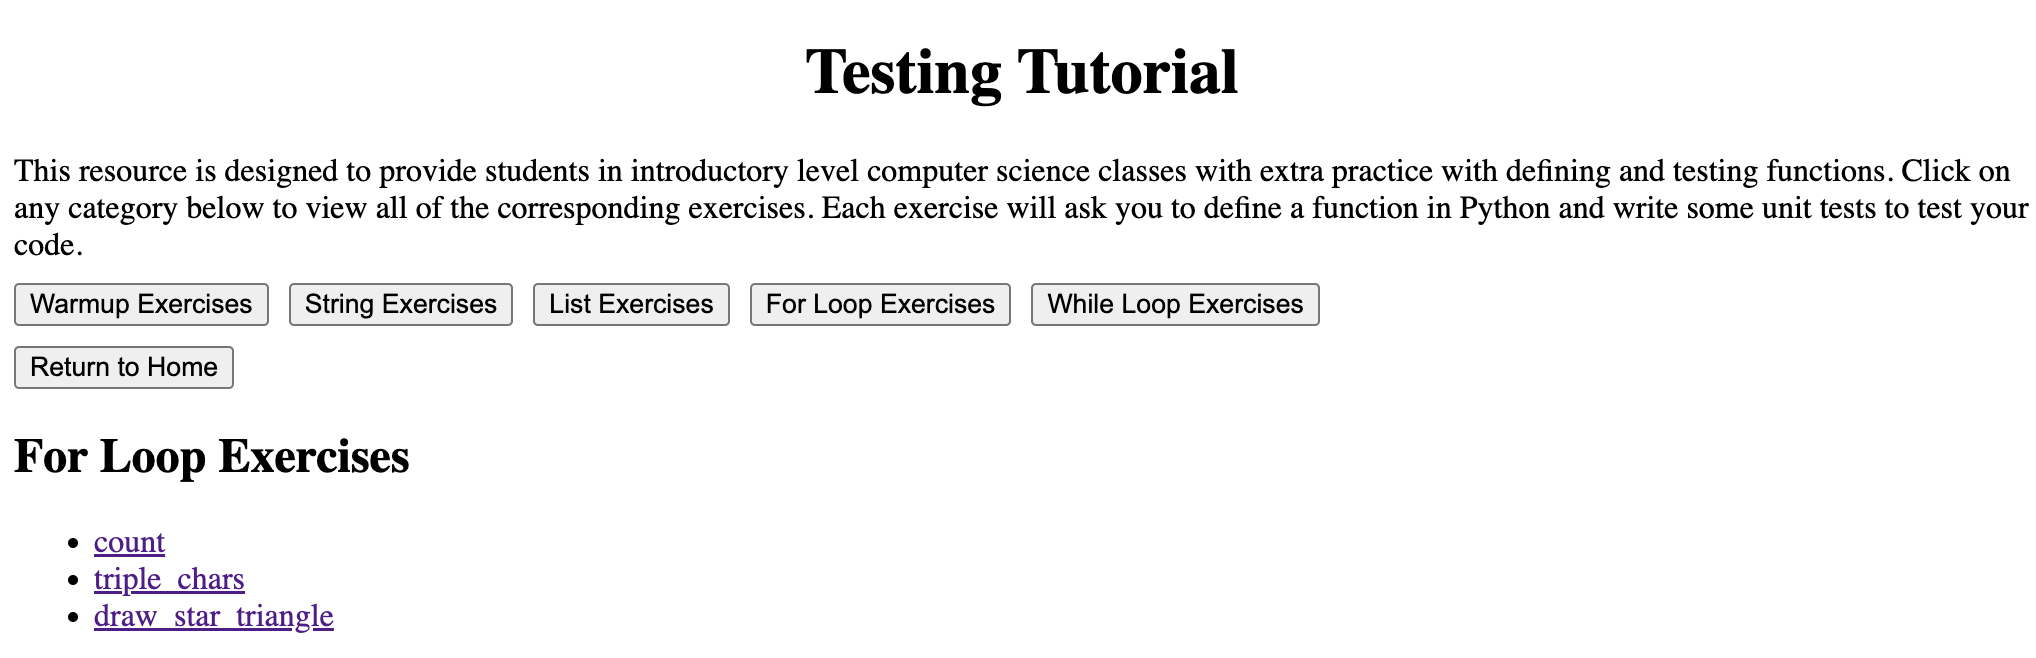
\includegraphics[width=.95\linewidth]{ForLoop.png}
    \caption{
        The three exercises in the \enquote{For Loop Exercises} category.
    }
    \label{fig:first-page}
\end{figure}

Selecting the count exercise leads to a page that explains the function to define, provides some example test cases with their expected outputs, has a text box with the function header in which to define the function, and has a table in which to write the test cases that displays the actual output and expected output after clicking “Run Tests”. This is shown in Figure 7.
\enquote{For Loop Exercises}.
\begin{figure}
    \centering
    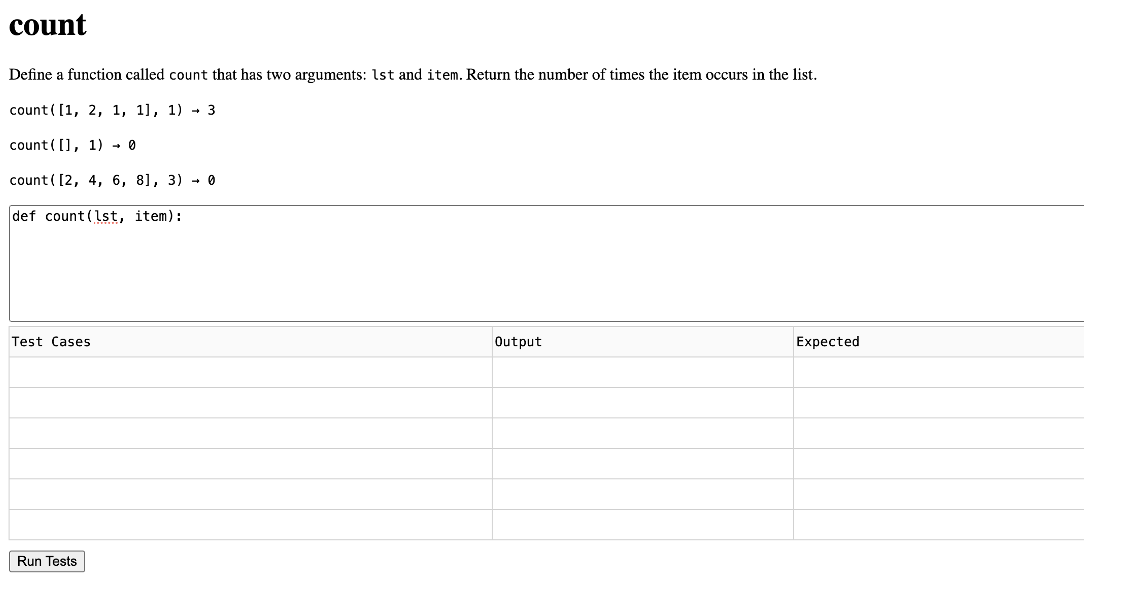
\includegraphics[width=.95\linewidth]{count.png}
    \caption{
        The count exercise.
    }
    \label{fig:first-page}
\end{figure}

When the function is defined and all of the rows have been filled in with test cases, the \enquote{Run Tests} button should be pressed. Test cases where the output matches the expected value are highlighted in green. Test cases where the output does not match the expected value are highlighted in red. (A selected cell in the table will turn white). As shown in Figure 8, this function has been defined incorrectly, so not all of the test cases pass.
\enquote{For Loop Exercises}.
\begin{figure}
    \centering
    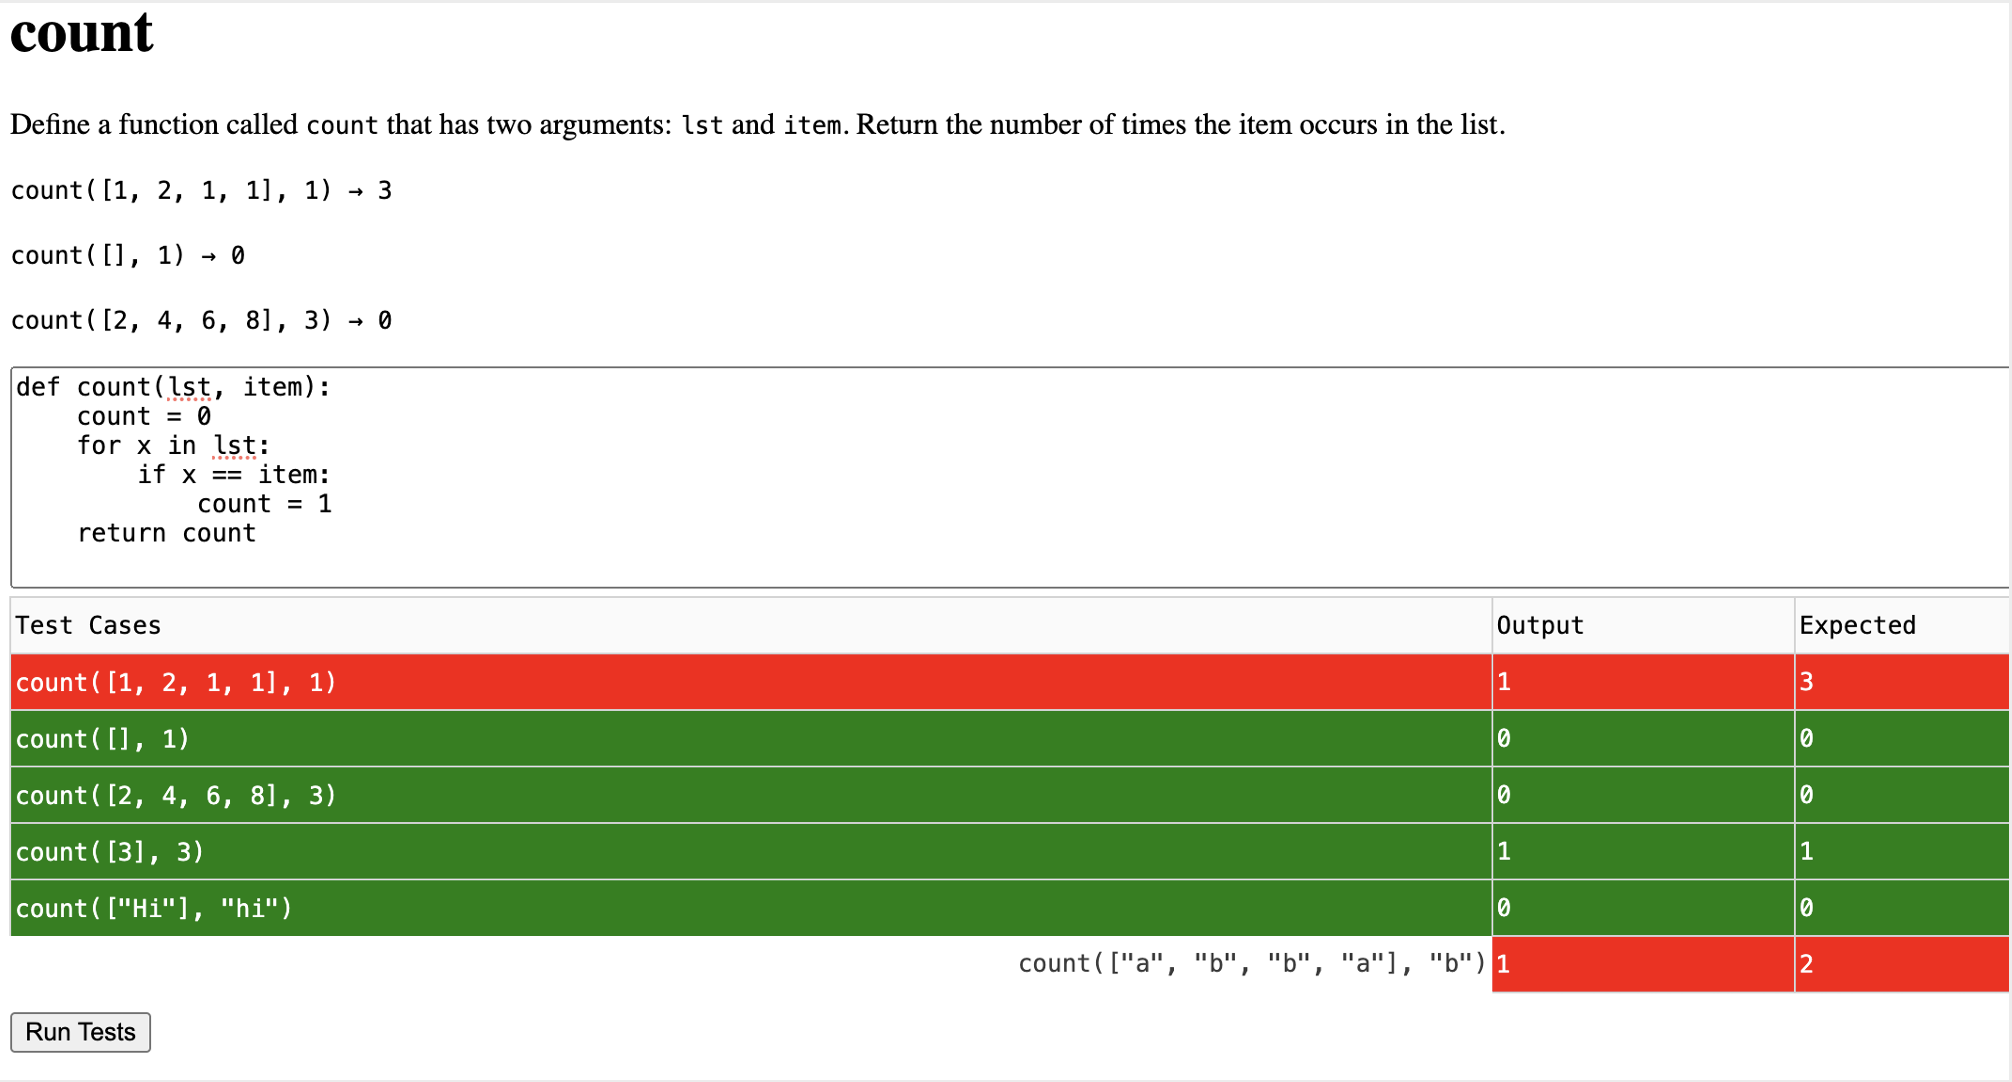
\includegraphics[width=.95\linewidth]{incorrect.png}
    \caption{
        The count function has been incorrectly defined.
    }
    \label{fig:first-page}
\end{figure}

The function can be edited until all of the test cases pass. In this case, the issue was that the count variable in the for loop was not being incremented by one, but was set to one. After fixing this issue, all of the test cases pass, as shown in Figure 9.
\enquote{For Loop Exercises}.
\begin{figure}
    \centering
    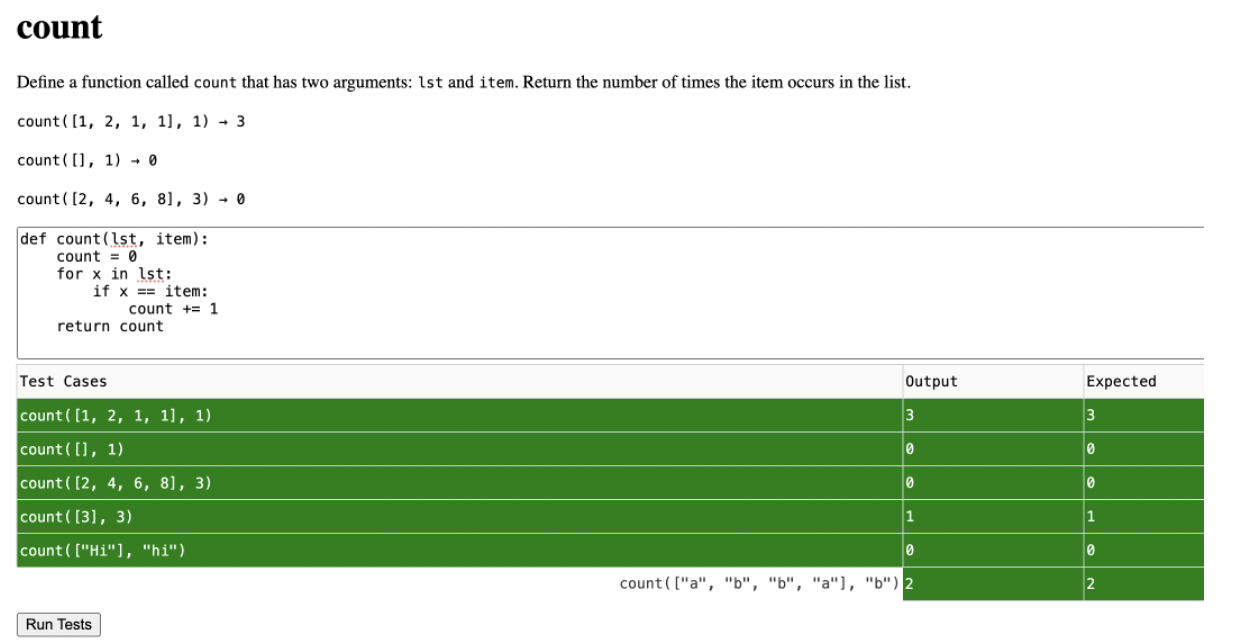
\includegraphics[width=.95\linewidth]{correct.png}
    \caption{
        The count function has been correctly defined.
    }
    \label{fig:first-page}
\end{figure}

Ultimately, the functionality of the website meets the core goals of this project. As outlined in the Method section, several different ideas were explored on how to handle the test case inputs. The AG Grid ended up being too complicated for what needed to be accomplished in this project \cite{AG}, so Dash's DataTable component was utilized. However, there is a lot of additional functionality that can be implemented to make this project even more in line with my original goals. 

\section{Ethical Considerations}

Although my intention was to design this project for beginners when it comes to coding and computer programming, I assumed a certain level of digital literacy when brainstorming this idea. However, this makes the resource inaccessible to a wide range of people. For instance, many high school graduates who did not take any computer science courses throughout their primary, secondary, and high school education may also not have had the necessary support systems to develop the digital literacy necessary to even begin learning how to code. Additionally, many people who completed their formal education before the existence of today’s technologies may not have the digital literacy necessary to undertake the process of learning about computer programming. According to a study on how older adults gain digital literacy via the use of tablet computers, “Even though there have been some recent gains in technology use, older adults are still the group the least likely to have crossed the digital divide… For example, in 2014, the overall Internet adoption rate in the United States was 87 [percent], while the adoption rate for people over 65 years old was only 57 [percent] (Pew Research Center, 2014).”\cite{Adults} These groups will face additional barriers to being able to make the most of an educational resource for coding compared to those that have benefited from a robust computer science and digital literacy education starting in primary school. Even if members of this latter group need support as they continue to build on their coding skills, they are more likely to know the existing resources available to them and how to overcome technology-related challenges. Additionally, they are more likely to have developed a certain amount of confidence when working with technology. Therefore, my project could very well be inaccessible to groups of people who perhaps need a free resource to learn foundational skills in computer programming, which is increasingly applicable to a large number of fields. As previously stated, my website is also not particularly suited for students who are not taking a Computer Science course, but are coding in a class in another department. Those students may find that my project does not give enough background information or guidance on the topic. 

There are also some security issues with my project. It only works if everything is handled carefully and nobody is trying to \enquote{break} my project. For instance, test cases must be typed correctly (using the correct function name), or they won't work. If a user messes up a test case, they may not be able to delete the incorrect character(s) and may have to start over. Additionally, my project makes use of the exec() function in the callback functions. There are some issues with the security surrounding this function. It can be used to \enquote{execute malicious code} and makes the \enquote{code more complex and difficult to understand}, which can make it inaccessible for people who could theoretically pick up this project in the future. However, if using it, there are certain steps that can be taken to make it safer, such as only passing \enquote{trusted inputs} to the exec() function, \enquote{using a debugger to step through the code}, and \enquote{testing the code to make sure that it is secure} \cite{Exec}. I have  made sure that only \enquote{trusted inputs} were passed and used a debugger while working on my project. 

Creating an educational resource is a large responsibility, and it was not feasible for me to adequately address all of the ethical considerations presented in this paper. This then leads to the conclusion that the important task of continuing to build and maintain an educational resource for computer science is best left up to a team of people with the expertise, time, and resources to ensure that they are doing everything possible to make this resource as accessible and user-friendly as possible. A large portion of the semester was devoted to me actually building the website, which unfortunately left little time for working on implementing additional features. I was not able to incorporate a lot of the feedback that I received from students and professors. Thus, it appears that it was not possible for me to effectively address all of the ethical concerns within the timeframe of a semester to a sufficient extent. While my project is a functional resource that students can use, there are many improvements that can be made to it before it is a product on the same scale as existing resources for Computer Science education.  

\printbibliography

\section{Appendix A: Replication Instructions}

This project relied on the Dash \cite{Dash} and Pandas packages (versions 2.18.0 and 2.2.2, respectively). The pages\_button.py file is what actually creates and runs the application, and all of the files in the pages folder contain the exercises (which all follow the same overall structure). If a new exercise is added, it will also need to be imported into the pages\_button.py file (from pages.file name import layout as file name\_layout) in order for it to be included in the app. Then, it will need to be added to the SUBPAGE\_LAYOUTS nested dictionary under the appropriate category of exercises. For example, if an exercise is in the \enquote{For Loop Exercises}, it should be added as \enquote{file name}: file name\_layout. Finally, it needs to be added to the CATEGORIES dictionary of lists under the appropriate category, as \enquote{For Loop Exercises}: [\enquote{file name}, ...].

\section{Appendix B: Code Architecture Overview}

As suggested in the previous sections, there are many ways to extend this project. For example, adding a log in feature so that a user's work can be saved is one of my top priorities when I continue working on this project. This will involve editing the pages\_button.py file. As previously stated, this project would certainly benefit from providing the user with more feedback on the test cases that they wrote. This will involve editing each file in the pages folder. Since each function is unique, the feedback itself will need to be specific to a given function. Therefore, this will involve make relatively significant changes to each file that cannot be copied over. Finally, adding more exercises to each category, as well as more categories, would provide users with more practice. As stated in Appendix A, adding a new file to the pages folder requires several simple changes to the pages\_button.py file. Overall, the main editing this project will envolve either (1) adding more files to the pages folder and updating the pages\_button.py file as necessary, (2) making edits only to the pages\_button.py file for changes to the overall app, or (3) making changes to existing files in the pages folder to make the project more accessible to users, which will generally not require changes to the pages\_button.py file.

\end{document}
